\documentclass[../main.tex]{subfiles}

\usepackage{float} % Librería para presentación de imágenes

\begin{document}

El dataset elegido guarda información recogida de la base de datos  European Antimicrobial Resistance Surveillance (EARS), en concreto la información relativa a aquellas bacterias que han desarrollado resistencia a los antiobióticos. El dataset se encuentra en el siguiente enlace: \href{https://www.kaggle.com/datasets/samfenske/euro-resistance}{kaggle.com/datasets/euro-resistance}. 

Cada una de las filas del dataset representa un estudio realizado sobre un grupo de personas. En las columnas se nos presenta la siguiente información sobre cada estudio:

\begin{itemize}
    \item Distribución: se refiere a si los datos se extrajeron de un género o grupo de edad en particular.
    \item RegionName: país de la institución informante.
    \item Tiempo: el año.
    \item  Categoría: grupo de edad o el género (dependiendo de la distribución).
    \item  Valor: porcentaje de bacterias que fueron resistentes al grupo de antibióticos.
    \item Bacterias: se refiere a las bacterias en las que se estudió la resistencia.
    \item Antibiótico: grupo de antibióticos que se usó para matar la bacteria.
\end{itemize}

En la imagen \ref{datasetSpy} se encuentra el dataset en formato .XMLSpy (tal cual se descarga de Kaggle).

\begin{figure}[ht]
    \centering
    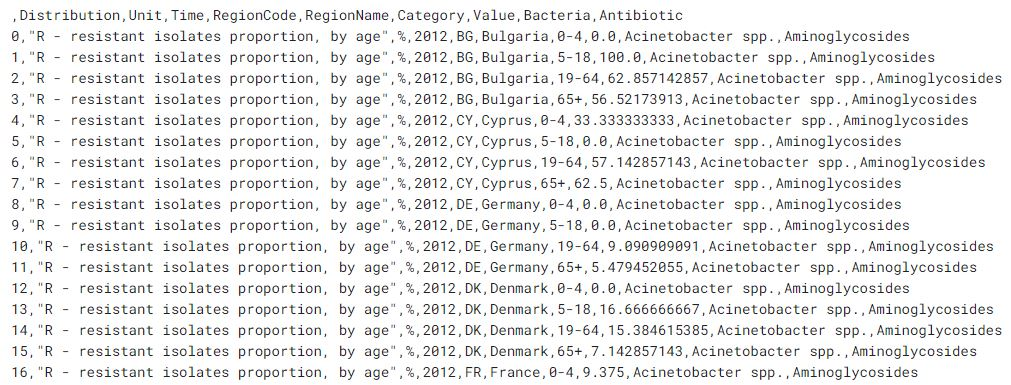
\includegraphics[scale=0.65]{dataseSpy}
    \caption{Dataset formato .XMLSpy}
    \label{datasetSpy}
\end{figure}


Se necesita que los datos estén en formato XML para poder realizar las distintas consultas y transformaciones. XML es un metalenguaje de marcado. Un lenguaje de marcado o lenguaje de marcas es una forma de codificar un documento que, junto con el texto, incorpora etiquetas o marcas que contienen información adicional acerca de la estructura del texto o su presentación Para ello se ha usado la siguiente herramienta online: \href{https://www.convertcsv.com/csv-to-xml.htm}{www.convertcsv.com}. Esta herramienta da como salida el archivo .XML de la imagen \ref{datasetXML}.

Como se puede observar en la imagen, se ha generado un nodo raíz, al que se ha llamado \textit{root}, y por cada fila del dataset se ha generado un nodo \textit{row}, el cual tiene como nodos hijos las columnas del dataset.

\begin{figure}[ht]
    \centering
    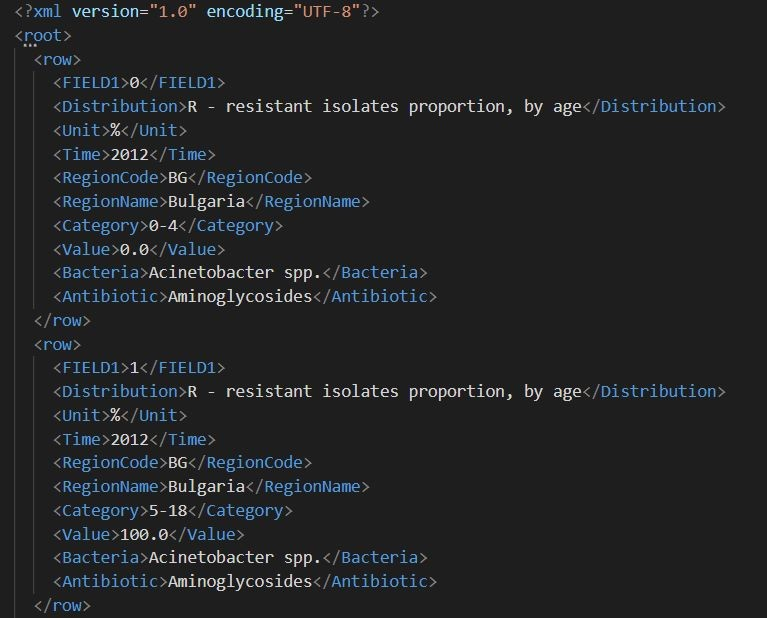
\includegraphics[width=0.7\textwidth]{datasetXML}
    \caption{Dataset formato .XML}
    \label{datasetXML}
\end{figure}

\end{document}